Se tiene un grafo dirigido con $n$ vértices y $m$ aristas. Tienes que encontrar un orden de los vértices, 
de modo que cada arista conduzca desde el vértice con un índice más pequeño a un vértice con uno más 
grande.

En otras palabras, desea encontrar una permutación de los vértices (orden topológico) que corresponda al orden definido por todas las aristas del grafo. Aquí hay un grafo dado junto con su orden topológico:

% TODO: \usepackage{graphicx} required
\begin{figure}[h!]
	\centering
	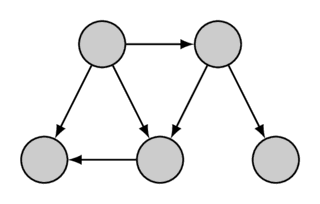
\includegraphics[width=0.35\linewidth]{img/topological_1}
	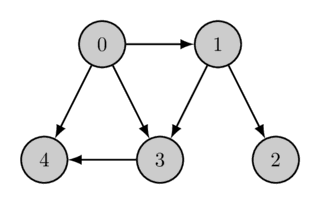
\includegraphics[width=0.35\linewidth]{img/topological_2}
	\label{fig:topological1}
\end{figure}
